\documentclass{beamer}
\usepackage{amsmath}
\usepackage{booktabs}
\usepackage{tikz}
\usetheme{default}
\title{A Synthetic Slide Workload}
\author{aiTeX qualification}
\date{September 2001}

\begin{document}
\begin{frame}
  \titlepage
\end{frame}

\begin{frame}{Mathematics and overlays}
  \begin{itemize}
    \item<1-> First deterministic point
    \item<2-> Second point with $\sum_{k=1}^{n}k=n(n+1)/2$
  \end{itemize}
\end{frame}

\begin{frame}{Tables and vectors}
  \begin{columns}
    \begin{column}{0.48\textwidth}
      \begin{tabular}{lr}
        \toprule Item & Value \\
        \midrule Alpha & 13 \\
        Beta & 21 \\
        \bottomrule
      \end{tabular}
    \end{column}
    \begin{column}{0.48\textwidth}
      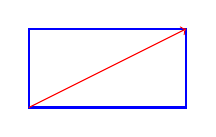
\begin{tikzpicture}
        \draw[blue,thick] (0,0) rectangle (2,1);
        \draw[red,->] (0,0) -- (2,1);
      \end{tikzpicture}
    \end{column}
  \end{columns}
\end{frame}
\end{document}
